% !TEX root =  ../main.tex


\begin{figure*}
\centering
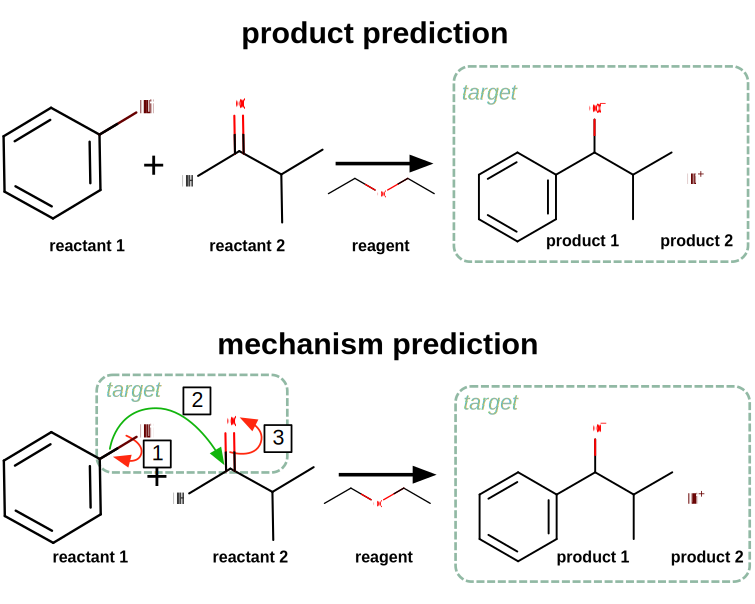
\includegraphics[width=\textwidth]{reaction_diagram}
\caption{a) The reaction prediction problem: Given the reactants and reagents, predict the structure of the product.}
\end{figure*}

In this section we describe the types of reactions we consider in this paper, and how it relates to previous work on reaction prediction. We then describe recent related work on deep graph models that inspire our model in the following section.

\paragraph{Chemical reactions.}
%In reality, the structure of a molecule is due to how electrons on each atom are interacting with each other. 

%% Bond localization?
Molecules consist of a set of atoms that are arranged into a structure by a set of bonds. 
As such, molecules can be depicted as a graph structure, where each node is an atom and each edge is a bond, 
as shown in Figure (note the convention that vertices which do not explicitly specify the atom name are assumed to be carbon C atoms). 

Each single bond represents the fact that two electrons are shared between the atoms that the bond connects\footnote{The vast majority of bonds in molecules are like this (so-called \emph{covalent} bonds), 
although our model also accommodates ionic bonds 
(in which one atom completely borrows the electrons of another atom and the atoms become charged.}.

%Molecules are broken and built via reactions. 
Just as electrons describe the current structure of molecules, they also describe how molecules react with other molecules to produce new ones. 
All chemical reactions involve the movement of electrons along paths of atoms in a set of reactant molecules. 
This movement causes the formation and breaking of chemical bonds that changes the reactants into a new set of product molecules.\footnote{This movement happens because it allows the set of molecules to move to a lower (and thus more favorable) energy state.} 
In this work, we will consider reactions that satisfy the following assumptions:
% \begin{enumerate}
% \item are single-step, so-called \emph{elementary} reactions.
% \item involve a pair of electrons, so-called \emph{heterolytic} reactions.
% \item either start with electrons on single atom, or with the electrons in an existing bond.
% \end{enumerate}
\begin{assumption}
Reactions are single-step\todo{MS:i am not sure this is really needed}, so-called \emph{elementary} reactions.
\label{assume:elem}
\end{assumption}

\begin{assumption}
Reactions involve pairs of electrons moving, so-called \emph{heterolytic} reactions.
\label{assume:het}
\end{assumption}

\begin{assumption}
Reactions either start with electrons on single atom (called \emph{free electrons}), or with the electrons in an existing bond.
\label{assume:atom_bond}
\end{assumption}

These sorts of reactions describe 81\% of \emph{organic reactions}\cite{herges1994coarctate} (i.e., reactions involving Carbon atoms) that have a large number of applications from drug design to the invention of new materials\cite{segler2018planning}\footnote{Organic reactions that do not satisfy these assumptions are homolytic reactions, and concerted reactions.}. 
%For this reason organic reactions has been the focus of recent work in reaction prediction in machine learning \cite{jin2017predicting,schwaller2017found}. 
Note that reactions which are multi-step can be decomposed into multiple single-step reactions in order to satisfy Assumption~\ref{assume:elem}.


\paragraph{Reactions as single electron paths.}
If reactions satisfy the above assumptions, then a chemical reaction is the result of pairs of electrons moving in a \emph{single path} through the reactant atoms. Further, this electron path will alternately remove existing bonds in molecules, and form new ones. We show this alternating structure in two example single-path reactions in Figure~\ref{fig:example}. In Figure~\ref{fig:example}(a) the reaction starts with the electrons in a bond, and in Figure~\ref{fig:example}(b) the reaction starts with the electrons in an atom. 

There are a number of benefits of predicting electron paths over predicting the outcomes of reactions directly (as in previous work \cite{jin2017predicting,schwaller2017found}):
\begin{itemize}
\item \textbf{Easy to interpret}: If the model makes a mistake, it is easy to see where it goes wrong by comparing the steps of the path with the correct steps.
\item \textbf{Sparse}: Reactions often only affect between 3 and 7 atoms out of anywhere from 10-50 reactant atoms. Modeling the reaction as a path allows us to exploit this sparsity.
\item \textbf{Chemical constraints}: Learning a path allows us to easily incorporate chemical constraints, such as the alternating removal and addition of bonds, among others.
\item \textbf{Compositionality}: Learning to combine lower-level abstractions of chemistry potentially allows to generalize better.
\end{itemize}